
\chapter{Traditional Advanced Control Strategies} \label{eca_chapter}
%\thispagestyle{fancy}

This chapter presents tools for the analysis and simulation of traditional advanced control strategies such as feedforward-feedback control, cascade control, among others that are currently under development.


\section{Feedforward-Feedback Control}

Consider el feedforward-feedback control system according to Fig. \ref{chp_eca_fig01_ff}.

\begin{figure}[H]
	\centering
	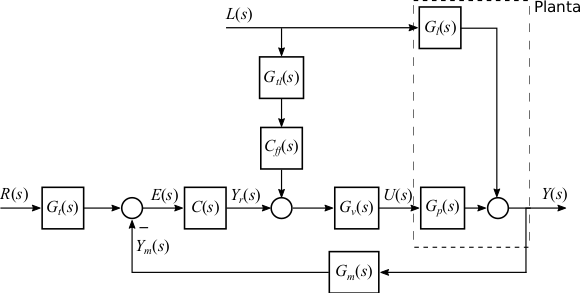
\includegraphics[scale=1.2]{./figuras/chapter_eca/controlFFFB.png}
	\caption{Feedforward-feedback control system.}
	\label{chp_eca_fig01_ff}
\end{figure}




\section{Cascade Control}

Consider the cascade control system according to Fig. \ref{chp_eca_fig01_ccd}.

\begin{figure}[H]
	\centering
	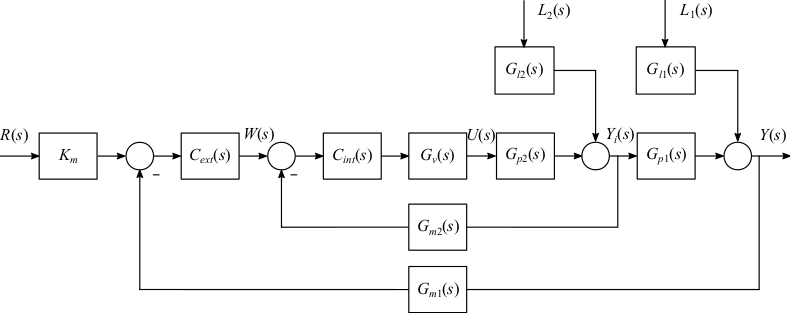
\includegraphics[scale=1.2]{./figuras/chapter_eca/controlCCD.png}
	\caption{Cascade control system.}
	\label{chp_eca_fig01_ccd}
\end{figure}



\section{Tools for Traditional Advanced Control Strategies}

\subsection{Analysis and Simulation of a Feedforward-Feedback Control System}

\textbf{Example 5.1}

Figure \ref{chpECA_fig01_ejemECA} shows the developed main window for traditional advanced control strategies that includes feedforward-feedback control and cascade control schemes.

\begin{figure}[H]
	\centering
	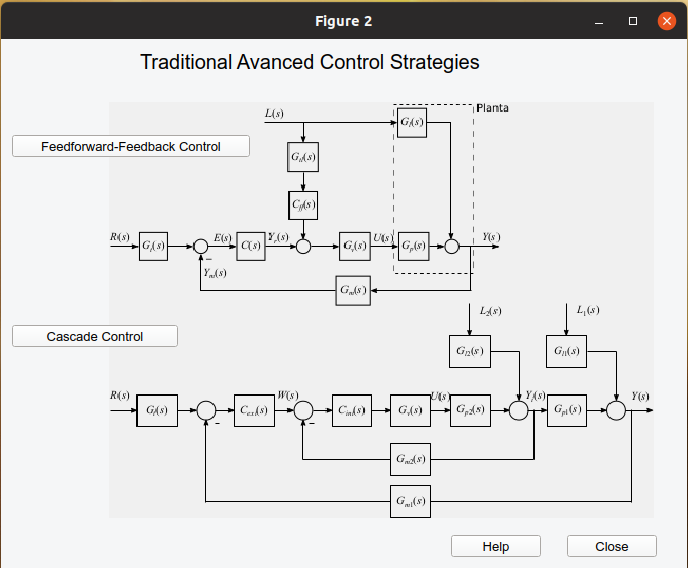
\includegraphics[scale=0.5]{./figuras/chapter_eca/fig01EjemECA.png}
	\caption{Main window for Traditional Advanced Control Strategies.}
	\label{chpECA_fig01_ejemECA}
\end{figure}

Figure \ref{chpECA_fig02_ejemECA} shows the developed main window to study the combined control scheme known as feedforward-feedback control.
\begin{figure}[H]
	\centering
	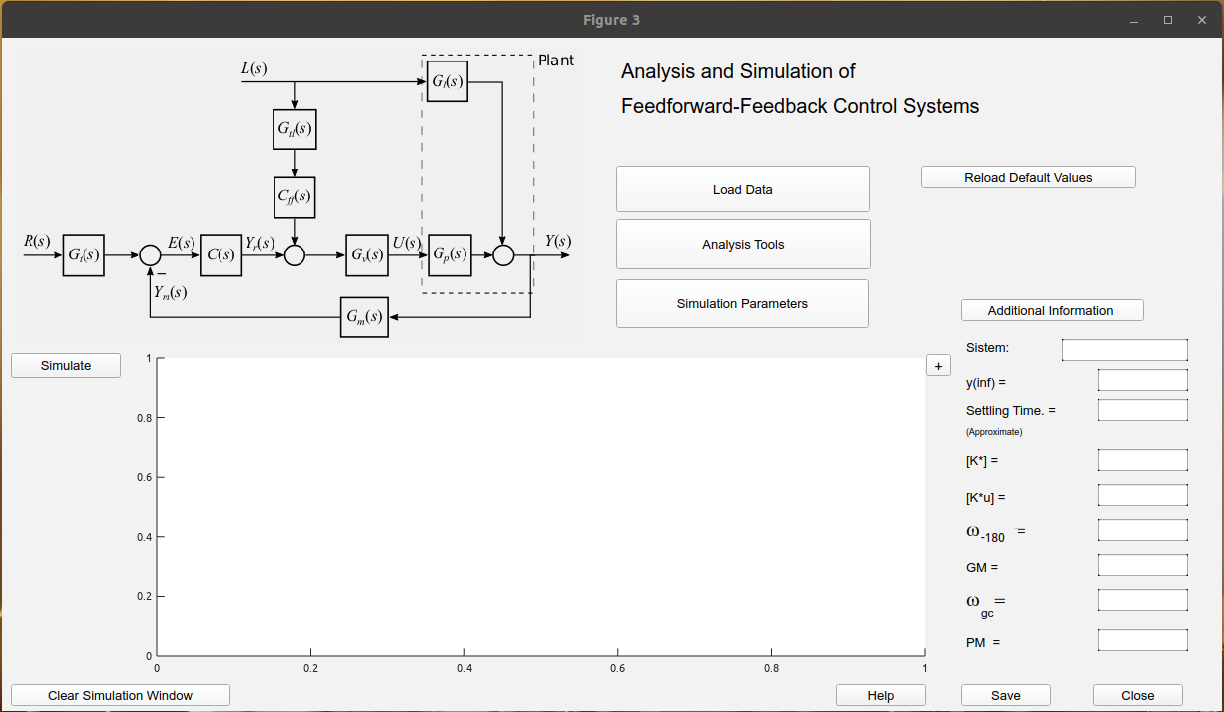
\includegraphics[scale=0.5]{./figuras/chapter_eca/fig02EjemECA.png}
	\caption{Main window for feedforward-feedback control.}
	\label{chpECA_fig02_ejemECA}
\end{figure}

Note that the load data bottom opens a window to load data for this example and it is similar to Fig. \ref{chp_lc_fig02_Gcl}.

Figure \ref{chpECA_fig03_ejemECA} shows the developed analysis tool window which is similar to developed window for closed loop system (Fig. \ref{chp_lc_fig03_Gcl}).
\begin{figure}[H]
	\centering
	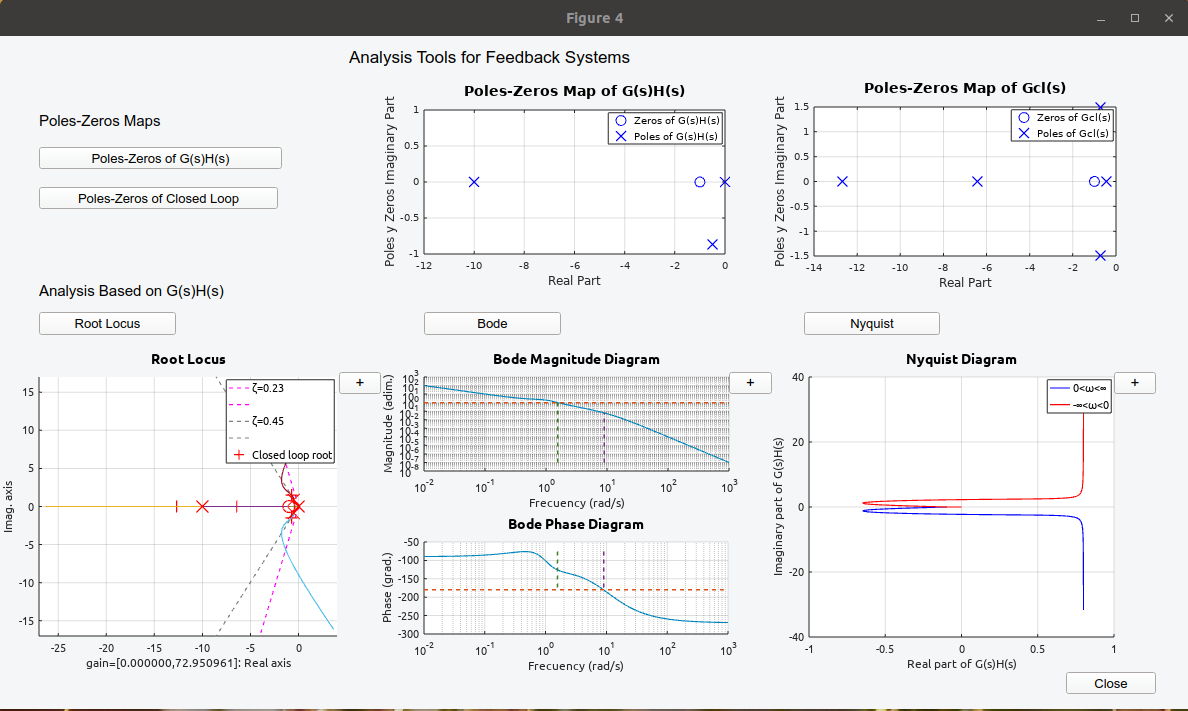
\includegraphics[scale=0.5]{./figuras/chapter_eca/fig03EjemECA.png}
	\caption{Analysis tool window for feedforward-feedback control system.}
	\label{chpECA_fig03_ejemECA}
\end{figure}

Finally, Fig. \ref{chpECA_fig04_ejemECA} shows the simulations obtained with this example.
\begin{figure}[H]
	\centering
	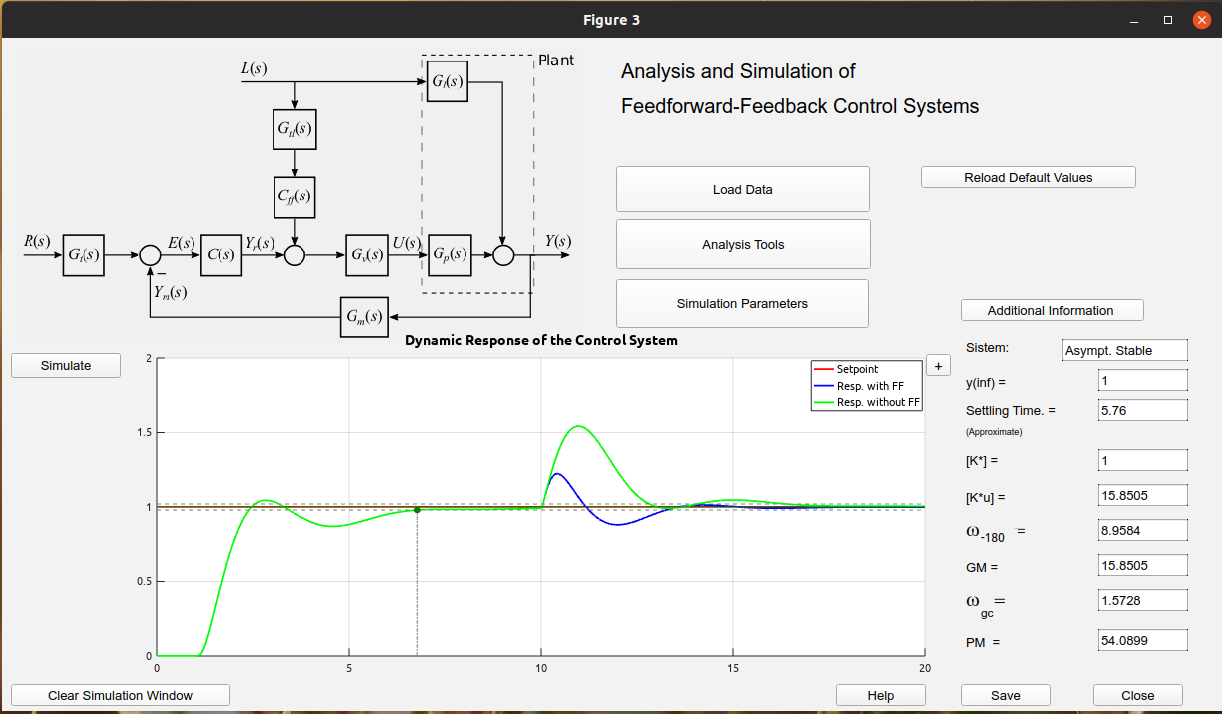
\includegraphics[scale=0.5]{./figuras/chapter_eca/fig04EjemECA.png}
	\caption{Simulation of feedforward-feedback control example.}
	\label{chpECA_fig04_ejemECA}
\end{figure}


\subsection{Analysis and Simulation of a Cascade Control System}

\textbf{Example 5.2}

If the user press the cascade control bottom indicated in Fig. \ref{chpECA_fig01_ejemECA} then, a window developed for cascade control scheme is opened. Figure \ref{chpECA_fig05_ejemECA} shows the developed main window to study this combined control scheme.

\begin{figure}[H]
	\centering
	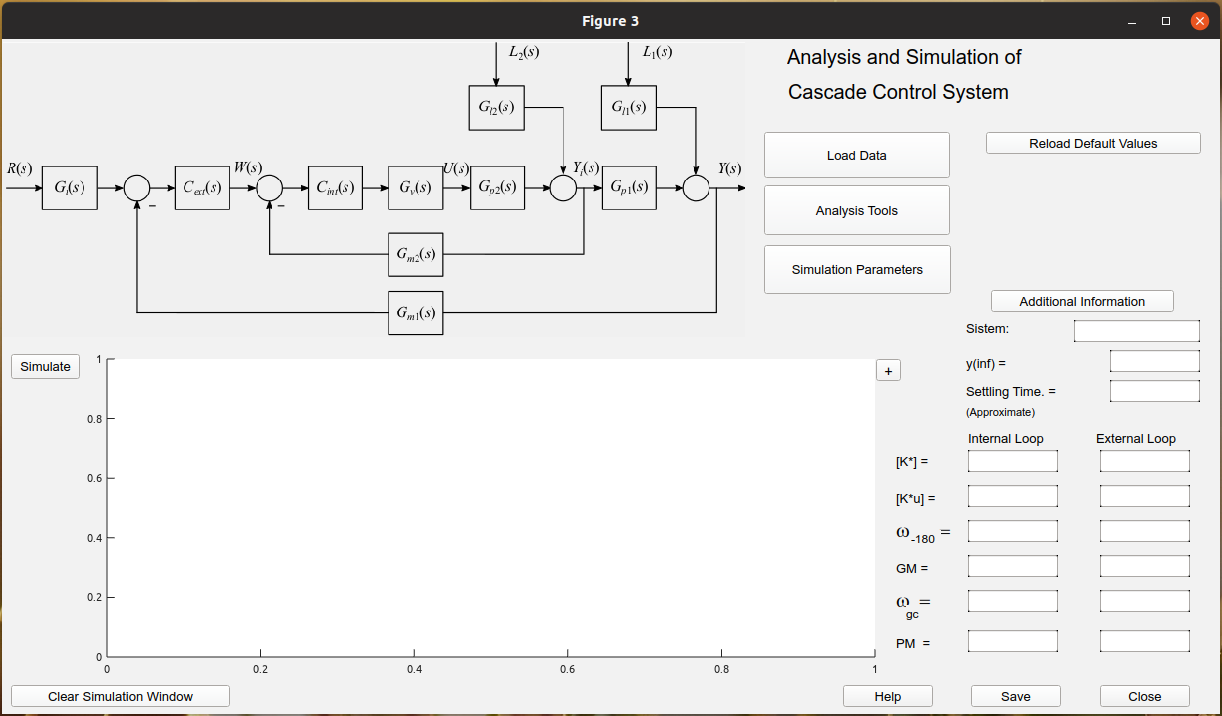
\includegraphics[scale=0.5]{./figuras/chapter_eca/fig05EjemECA.png}
	\caption{Main window for cascade control.}
	\label{chpECA_fig05_ejemECA}
\end{figure}

Note that the load data bottom opens a window to load data for this example and it is similar to Fig. \ref{chp_lc_fig02_Gcl}. Also, when de bottom analysis tools is pressed the window indicated in Fig. is opened.

\begin{figure}[H]
	\centering
	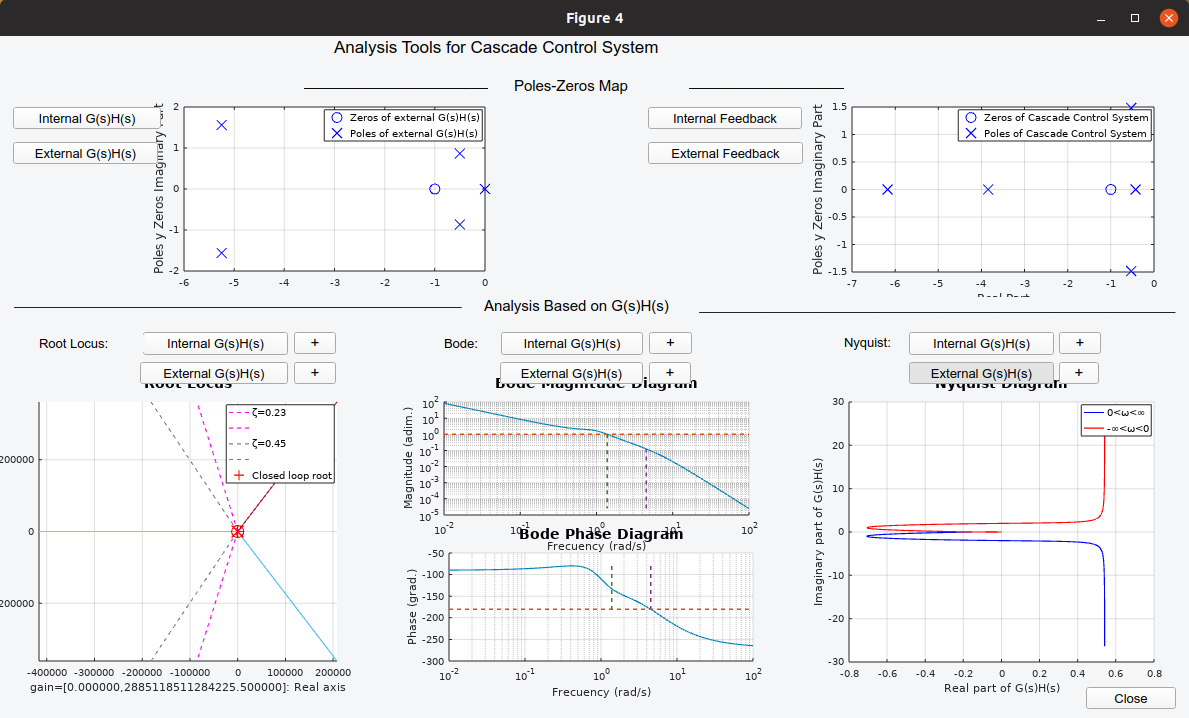
\includegraphics[scale=0.5]{./figuras/chapter_eca/fig06EjemECA.png}
	\caption{Analysis tool window for control control system.}
	\label{chpECA_fig06_ejemECA}
\end{figure}

Note that in mentioned window, the user can study internal and external loop independently.  

Finally, Fig. \ref{chpECA_fig07_ejemECA} shows the simulations obtained with this example.
\begin{figure}[H]
	\centering
	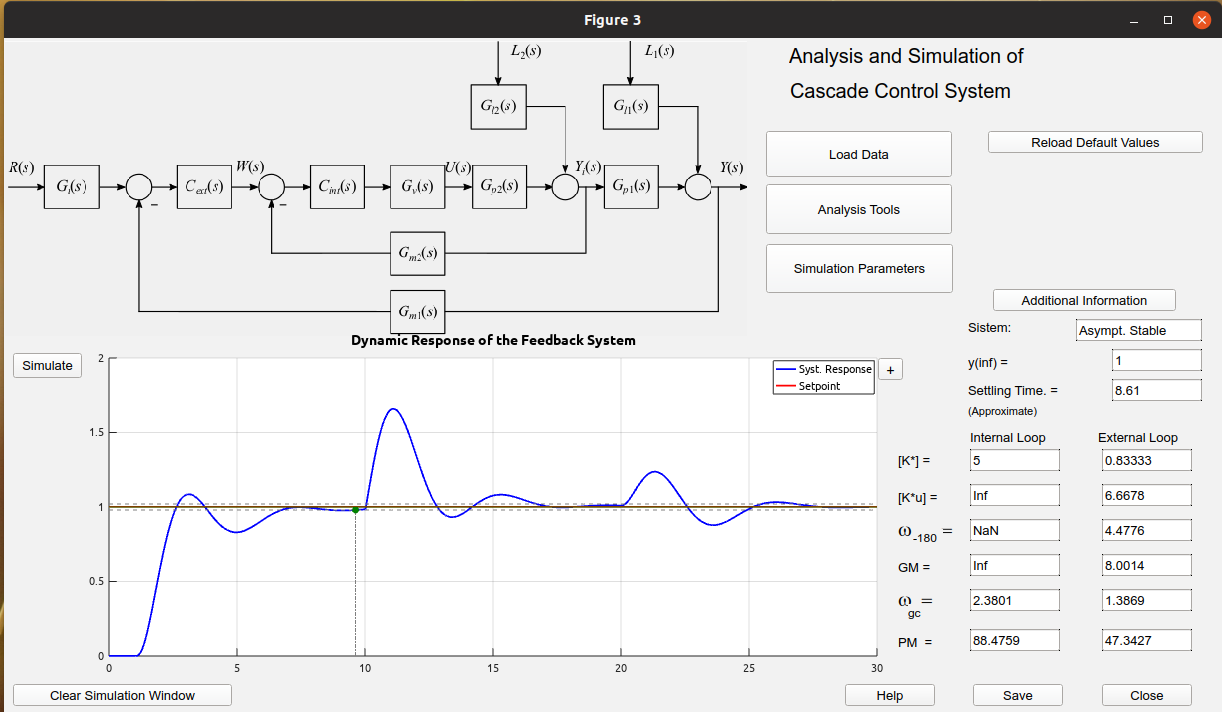
\includegraphics[scale=0.5]{./figuras/chapter_eca/fig07EjemECA.png}
	\caption{Simulation of cascade control example.}
	\label{chpECA_fig07_ejemECA}
\end{figure}


\section{Conclusions}


